\section{Problem set 2}
\subsection{Preface}
This problem set provided an introduction to simple pseudorandom number
generator called ,,linear-feedback shift register'' (LSFR) which is a shift
register whose input bit is a linear function of it's previous state. The goal
of this problem set was to get familiar with LSFR structure, analyze it's possible
input - initialization vector - and output generated using different IVs.

\subsection{Assignment 1}
The goal of this task was to analyze and sketch out architectures of the
\texttt{LSFR} entity provided by the lecturer.

\begin{figure}[!htb]
  \center{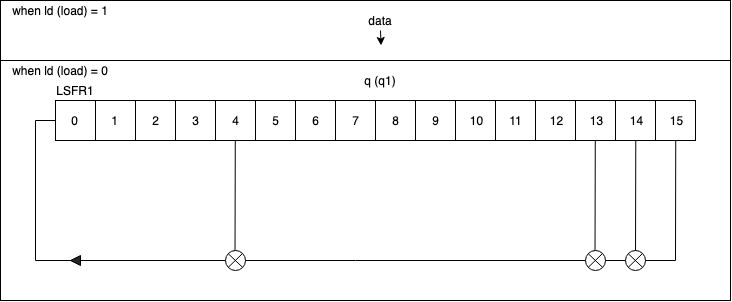
\includegraphics[scale=0.5]
  {drawings/lsfr_first.png}}
  \caption{\label{fig:assignment1-lsfr_first} Architecture \texttt{first} of \texttt{LSFR}.}
\end{figure}

\begin{figure}[!htb]
  \center{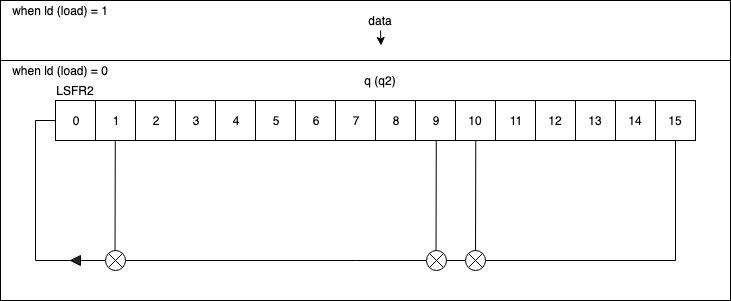
\includegraphics[scale=0.5]
  {drawings/lsfr_second.png}}
  \caption{\label{fig:assignment1--lsfr_second} Architecture \texttt{second} of \texttt{LSFR}.}
\end{figure}


\subsection{Assignment 2}
\subsection{Assignment 3}
\subsection{Assignment 4}
\subsection{Assignment 5}